\documentclass[12pt,prb,reprint]{revtex4-1}
%% \documentclass[12pt,prb,reprint]{elsarticle}
\usepackage{xcolor}
\usepackage{amsmath}
\usepackage{graphicx}
\usepackage[normalem]{ulem}

\begin{document}


\title{Summary of Mueller, Froyen and AFLOW kpoint tests}

\author
{Wiley S. Morgan}
\affiliation
{Department of Physics and Astronomy, Brigham Young University, Provo Utah 84602 USA}

\author
{Gus L. W. Hart}
\affiliation
%% \address
{Department of Physics and Astronomy Brigham Young University, Provo Utah 84602 USA}


\begin{abstract}

\end{abstract}

\maketitle

\section{Introduction} \label{Intro}

In computational materials science many materials properties are
determined by performing integrals over the Brillouin zone. The
accuracy of these calculations is directly related to the symmetries
and densities of reciprocal space points (k-points) used to perform
the integral. Over the years there have been many attempts to
streamline the development of the most efficient k-point sampling so
that a researcher can perform efficient calculations without having to
spend time determinig what the best k-point grid is. The most recent
advancement in this effort, contributed by Wisesa et al.\cite{Wisesa},
employed informatics to do a brute force search over possible k-point
grids.

With this new database avaialble the question becomes how much better
are these grids than those typically used in research today? To
answere that question we have performed convergence tests for nine
pure elements (Al, Cu, K, Pd, Re, Ti, V, W, and Y) using the
generalized Monkhorst-Pack (GMP) k-points developed by Wisesa,
AFLOW\cite{AFLOW} and the Froyen\cite{Froyen} k-point method in
VASP. These tests will demonstrate where the methad developed by
Wisesa has advantages over other methods currently employed.

\section{Methodology} \label{Method}

In order to generate the POSCARs for the VASP calculations we
enumerated\cite{enum3} a binary system of each parent lattice for each
element. For the cubic parent lattices we enumerated cell sizes from 1
to 11 and for the hexagonal close packed (HCP) parent lattices we en
umerated cell sizes from 1 to 7 (in HCP there are 2 atoms in the basis
so this is equivalent to having a range of 2 to 14 atoms in the
cells). We then selected a cell at random from the enumerated list for
each atomic species at each cell size to create our test pool.

We used PAW\_PBE potentials with the POTCARS constructed so that both
of the binary elements would have the same potential. For the Froyen
and the GMP k-point tests the number of ionic steps was limited to
20. The AFLOW k-point tests used the default values for metals built
into the AFLOW framework.

\subsection{K-point generation} \label{k-grid}

For each POSCAR selected VASP calculations were performed with k-point
grids of densities 3 to 22 cubed k-points per reciprical atom. For
AFLOW and the GMP k-point grids it was sufficient to specify the
desired number of k-points in the input files and allow the codes to
generate the appropriate k-point grids. For the Froyen method grids
had to be generated by hand for the most common k-point lattices that
were commencerate with the parent lattice. That is for the cubic
parent lattices k-point grids that had simple cubic, face-centered
cubic, and body-centered cubic lattices were used with on offset from
gamma of (0.5, 0.5, 0.5) while for the HCP parent lattice 4 different
HCP k-point grids were generated each having a different offset from
gamma (the offsets for the 4 cases were HCP1: (0.5, 0.5, 0.0), HCP2:
(0.0, 0.0, 0.5), HCP3: (0.5, 0.5, 0.5), and HCP4: (0.0, 0.0, 0.0)).

Each system was allowed only a single run of the VASP code to
relax. For the cubic elements the converged energy value was
considered to be the energy of a single atom cell with 22 cubed
kpoints per reciprocal atom. For the elements that have a HCP parent
lattice the converged energy was considered to be the average energy
found from all four offstets at the highest k-point density for the
Froyen cases. {\color{red}Since the converged energy for the HCP cases is an
average value we have excluded any VASP calculations that converged to
within a standard deviation of the averaged energy from our dataset.}

\section{Comparison of Methods} \label{comparison}

All results from the VASP calculations can be found in
Fig.~\ref{fig:AllvGMP}. The figure displays the error in the enery
calculated vs the ratio of irreducible k-points from a method relative
to GMP. For example to get an error of 1E-3 in the energy calculation
a Froyen BCC or FCC grid would need 100 times as many irreducible
k-points as GMP. From this plot we can clearly see that for cubic
systems the GMP vastlp outperforms any other method in use. However,
when we consider the HCP systems we see a drastic drop in
performance. In order to better understand this trend we investigate
the k-points selected by GMP for these systems.

\begin{figure} %% [h]
  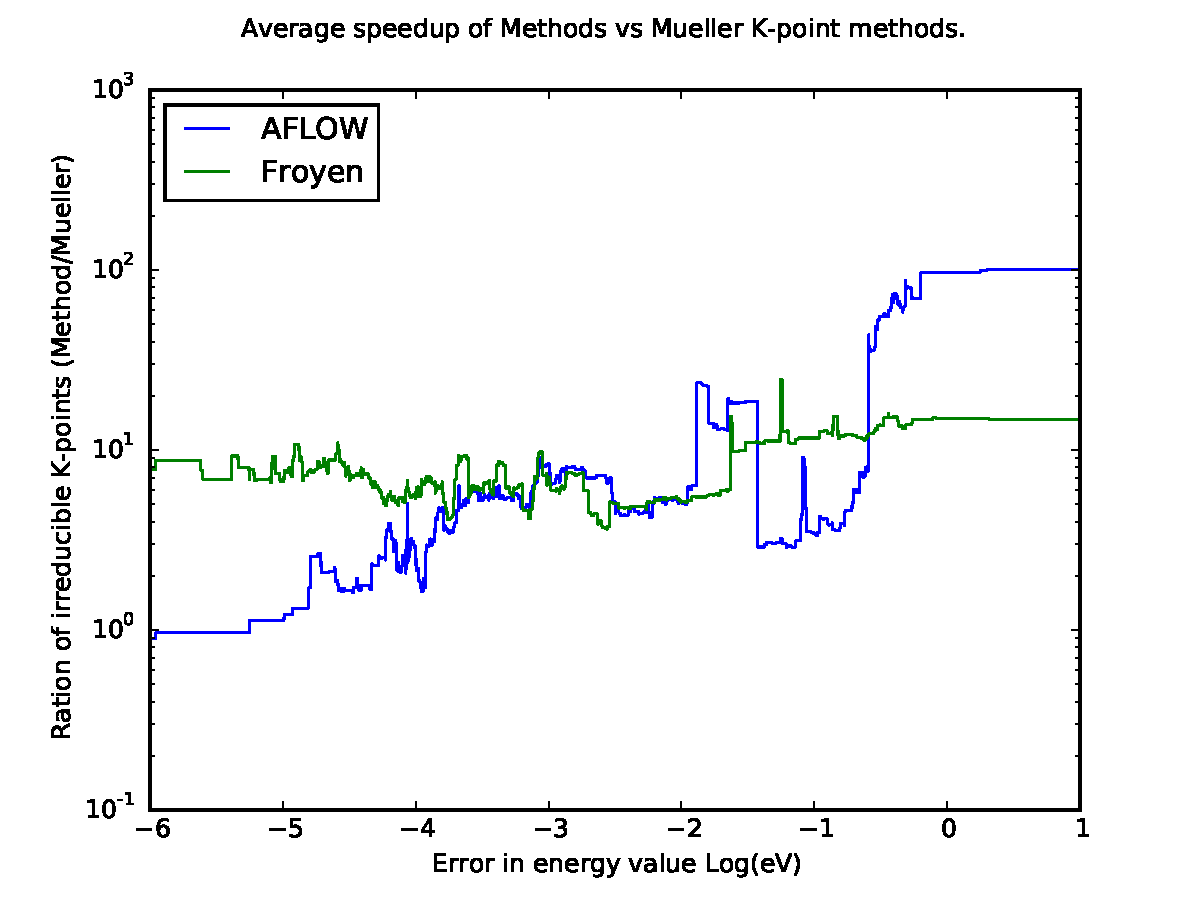
\includegraphics{../plots/All_vs_Mueller.pdf}
  \centering
  \caption{A plot of the convergence of the different k-point selction
    methods as compared to GMP. The error in the energy relative to
    the converged value is displayed on the x-axis. The y-axis relates
    the ratio of the number of irreducible k-points needed to reach
    the desired accuracy.}
  \label{fig:AllvGMP}
\end{figure}

\section{Investigation of HCP} \label{HCP}

As we saw in Sec.~\ref{comparison} GMP does not perform as well for
HCP grids as it does for other systems. In order to unerstand this
better we will study the k-points selected by GMP for a 2-atom HCP
cell at a number of k-point densities. For ease of analysis we will
investigate GMP grids that include the gamma point. For the
investigation we will look at k-point densities of 64 and 512 k-points
in the integration cell.

In the case of 64 k-points GMP provides the following k-points in
reciprocal coordinates:

$0.00000000000000 0.00000000000000 0.00000000000000 1.0 ! 1$
$0.25000000000000 0.62500000000000 0.50000000000000 4.0 ! 2$
$0.50000000000000 0.25000000000000 0.00000000000000 2.0 ! 3$
$0.00000000000000 0.50000000000000 0.00000000000000 1.0 ! 4$

These vectors are all linearly dependent, that is
$(0.5,0.25,0)=2*(0.25,0.625,0.5) mod 1$, where the mod 1 maps the new
vector back inside the cell. We can then conclude that the vector
$(0.25,0.625,0.5)$ is a basis vector for this grid since all other
points can be constructed from it. The other two vectors in the basis
must simultaneasly be able to map k-points back into the cell and be
equivalent to a provided point (otherwise they would point to
additional k-points in the irreducible zone). These basis for this
grid must there be:

$(0.25,0.625,0.5)$
$(1,0,0)$
$(0,0,1)$

Now that we have a basis for this grid we want to ensure that the grid
preserves the symmetry of the original parent lattice and that the
ratio of reducible k-points to irreducible k-points is less than the
total number of symmetry operations for the parent cell. The first
check will ensure that the provided grid will have the maximal
possible reduction of k-points for the cell. The second will verify
that the reduction we see is appropriate for the system.

In order to verify the first condition we need to review some basics
of group theory and the symmetry group. Each crystal class has a point
group $G$ that contains all the symmetries of the crystal. Hexagonal
lattices have a point group consiting of 24 different operations. Each
of these 24 operations can be recustructed from the generators $Gs$ of
the point group by taking all possible combinations of the
generators. The point group can take multiple forms but here we will
consider that each operation is a matrix that acts on a vector
expressed in cartesian coordinates.

\section{Conclusion} \label{conclusion}

\section{Acknowledgements}
This work was supported under: ONR (MURI N00014-13-1-0635).

\section{References}

\bibliographystyle{unsrt}
\bibliography{kp}

\end{document}
